% ============================================================
%  Chapter 7 — Quantum Statistics and the Grand Canonical Ensemble
%  Merged from parts 16, 17, and 19.
% ============================================================

\chapter{Quantum Statistics and the Grand Canonical Ensemble}

% ------------------------------------------------------------------
\section{Quantum Particles: Bosons and Fermions}
% ------------------------------------------------------------------

\begin{definition}[Bosons and Fermions]
\textbf{Fermions} have half-integer spin; their many-body wavefunction is
\emph{antisymmetric} under exchange of any two particles.  \textbf{Bosons}
have integer spin; their wavefunction is \emph{symmetric} under exchange.
\end{definition}

The properly symmetrised two-particle wavefunctions are
\begin{align}
    \text{Bosons:}\quad
    \Psi_{k_1k_2}
    &= \frac{1}{\sqrt{2}}\!\left[\psi_{k_1}(1)\psi_{k_2}(2)
       +\psi_{k_2}(1)\psi_{k_1}(2)\right],\\
    \text{Fermions:}\quad
    \Psi_{k_1k_2}
    &= \frac{1}{\sqrt{2}}\!\left[\psi_{k_1}(1)\psi_{k_2}(2)
       -\psi_{k_2}(1)\psi_{k_1}(2)\right].
\end{align}
For fermions the wavefunction vanishes when $k_1 = k_2$: this is the
\textbf{Pauli exclusion principle}.

\begin{fact}
Bosons: $n_k = 0, 1, 2, \ldots$ (unrestricted).
Fermions: $n_k \in \{0, 1\}$ only.
\end{fact}

States are labelled by occupation numbers $|n_1, n_2, \ldots\rangle$ with $\sum_i n_i = N$; $E = \sum_i \varepsilon_i n_i$.

The canonical $Z_N$ cannot be factored because occupations are coupled by $\sum n_i = N$. The approximation $Z_N \approx Z_1^N/N!$ requires typical occupancies $\ll 1$; at lower $T$ we need the grand canonical framework.

\begin{example}
Three bosons among harmonic oscillator levels with energies $(k+\tfrac{1}{2})\hbar\omega$:
the microstates are tuples $(n_0,n_1,n_2,\ldots)$ with $\sum n_i = 3$.
Three fermions cannot all occupy the lowest level; the Pauli principle forces
filling the lowest three available spin-states.

\begin{center}
\begin{tikzpicture}[scale=0.85]
  \foreach \lv in {0,1,2,3} {
    \draw[gray] (0, \lv*0.8) -- (1.4, \lv*0.8);
  }
  \filldraw[blue!70!black] (0.35, 0.0) circle (3pt);
  \filldraw[blue!70!black] (0.70, 0.0) circle (3pt);
  \filldraw[blue!70!black] (1.05, 0.0) circle (3pt);
  \node[below, font=\small] at (0.70, -0.15) {$(3,0,0,0)$};
  \node[above, font=\scriptsize] at (0.70, 2.55) {$E=\tfrac{3}{2}\hbar\omega$};

  \foreach \lv in {0,1,2,3} {
    \draw[gray] (2.0, \lv*0.8) -- (3.4, \lv*0.8);
  }
  \filldraw[blue!70!black] (2.70, 0.0) circle (3pt);
  \filldraw[blue!70!black] (2.70, 0.8) circle (3pt);
  \filldraw[blue!70!black] (2.70, 1.6) circle (3pt);
  \node[below, font=\small] at (2.70, -0.15) {$(1,1,1,0)$};
  \node[above, font=\scriptsize] at (2.70, 2.55) {$E=\tfrac{7}{2}\hbar\omega$};

  \foreach \lv in {0,1,2,3} {
    \draw[gray] (4.0, \lv*0.8) -- (5.4, \lv*0.8);
  }
  \filldraw[blue!70!black] (4.50, 0.0) circle (3pt);
  \filldraw[blue!70!black] (4.90, 0.0) circle (3pt);
  \filldraw[blue!70!black] (4.70, 0.8) circle (3pt);
  \node[below, font=\small] at (4.70, -0.15) {$(2,1,0,0)$};
  \node[above, font=\scriptsize] at (4.70, 2.55) {$E=\tfrac{5}{2}\hbar\omega$};

  \node[left, font=\scriptsize] at (-0.1, 0.0) {$\varepsilon_0$};
  \node[left, font=\scriptsize] at (-0.1, 0.8) {$\varepsilon_1$};
  \node[left, font=\scriptsize] at (-0.1, 1.6) {$\varepsilon_2$};
  \node[left, font=\scriptsize] at (-0.1, 2.4) {$\varepsilon_3$};
  \draw[->] (-0.1, -0.3) -- (-0.1, 3.0) node[above, font=\small] {$E$};
  \node[above, font=\small\bfseries] at (2.70, 3.1) {Boson configurations ($N=3$)};
\end{tikzpicture}\\[3pt]
{\small\itshape Bosons: multiple particles may occupy the same energy level.}
\end{center}
\end{example}

% ------------------------------------------------------------------
\section{The Grand Canonical Ensemble}
% ------------------------------------------------------------------

Abandoning fixed $N$, the system exchanges both energy and particles with a reservoir.

\begin{definition}[Grand Canonical Ensemble]
The system exchanges energy and particles with a reservoir at temperature $T$
and chemical potential $\mu$.  Fixed: $V$, $T$, $\mu$.  Fluctuating:
$U$, $N$ (only averages $\langle U\rangle$, $\langle N\rangle$ are determined
by the reservoir).
\end{definition}

\begin{center}
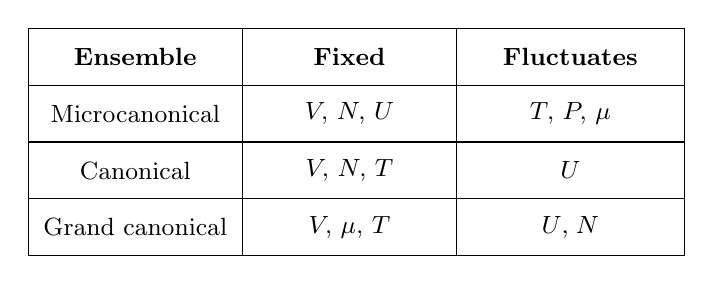
\begin{tikzpicture}[scale=0.85]
  \def\cA{0}   \def\cB{3.2} \def\cC{6.4} \def\cD{9.8}
  \def\rTop{0} \def\rOne{-0.85} \def\rTwo{-1.70}
  \def\rThree{-2.55} \def\rBot{-3.40}
  \foreach \y in {\rTop, \rOne, \rTwo, \rThree, \rBot} {
    \draw (\cA, \y) -- (\cD, \y);
  }
  \foreach \x in {\cA, \cB, \cC, \cD} {
    \draw (\x, \rTop) -- (\x, \rBot);
  }
  \node[font=\small\bfseries] at ({(\cA+\cB)/2}, {(\rTop+\rOne)/2}) {Ensemble};
  \node[font=\small\bfseries] at ({(\cB+\cC)/2}, {(\rTop+\rOne)/2}) {Fixed};
  \node[font=\small\bfseries] at ({(\cC+\cD)/2}, {(\rTop+\rOne)/2}) {Fluctuates};
  \node[font=\small] at ({(\cA+\cB)/2}, {(\rOne+\rTwo)/2}) {Microcanonical};
  \node[font=\small] at ({(\cB+\cC)/2}, {(\rOne+\rTwo)/2}) {$V,\,N,\,U$};
  \node[font=\small] at ({(\cC+\cD)/2}, {(\rOne+\rTwo)/2}) {$T,\,P,\,\mu$};
  \node[font=\small] at ({(\cA+\cB)/2}, {(\rTwo+\rThree)/2}) {Canonical};
  \node[font=\small] at ({(\cB+\cC)/2}, {(\rTwo+\rThree)/2}) {$V,\,N,\,T$};
  \node[font=\small] at ({(\cC+\cD)/2}, {(\rTwo+\rThree)/2}) {$U$};
  \node[font=\small] at ({(\cA+\cB)/2}, {(\rThree+\rBot)/2}) {Grand canonical};
  \node[font=\small] at ({(\cB+\cC)/2}, {(\rThree+\rBot)/2}) {$V,\,\mu,\,T$};
  \node[font=\small] at ({(\cC+\cD)/2}, {(\rThree+\rBot)/2}) {$U$,\;$N$};
\end{tikzpicture}\\[3pt]
{\small\itshape The three standard ensembles and their fixed vs.\ fluctuating quantities.}
\end{center}

\subsection{Derivation of the Grand Canonical Distribution}

For microstate $j$ (energy $E_j$, particles $N_j$), $P_j \propto \Omega_R(U_\text{tot}-E_j, N_\text{tot}-N_j)$. Taylor-expanding the reservoir entropy:
\begin{align}
    S_R(U_\text{tot} - E_j,\, N_\text{tot} - N_j)
    &\approx S_R(U_\text{tot}, N_\text{tot})
      - E_j\left.\pdv{S_R}{U}\right|_N
      - N_j\left.\pdv{S_R}{N}\right|_U.
\end{align}
Using $(\partial S_R/\partial U)_N = 1/T$ and $(\partial S_R/\partial N)_U = -\mu/T$
and exponentiating:

\begin{formula}
\begin{equation}
    P_j(E_j, N_j) = \frac{1}{\mathcal{Z}}\,e^{-\beta(E_j - \mu N_j)},
\end{equation}
\end{formula}
where $\beta = 1/k_BT$ and $\mathcal{Z}$ is fixed by normalisation.

\begin{definition}[Grand Partition Function]
\begin{equation}
    \mathcal{Z} = \sum_j e^{-\beta(E_j - \mu N_j)} = \sum_j e^{-\beta E_j}\,e^{\beta\mu N_j}.
\end{equation}
\end{definition}

\subsection{Grand Potential and Thermodynamic Derivatives}

\begin{definition}[Grand Potential]
\begin{equation}
    \Omega \equiv -k_BT\ln\mathcal{Z} = U - TS - \mu N,
    \qquad d\Omega = -S\,dT - P\,dV - N\,d\mu.
\end{equation}
\end{definition}

\begin{formula}
\begin{equation}
    S = -\left.\pdv{\Omega}{T}\right|_{V,\mu}, \qquad
    P = -\left.\pdv{\Omega}{V}\right|_{T,\mu}, \qquad
    \langle N\rangle = -\left.\pdv{\Omega}{\mu}\right|_{T,V}.
\end{equation}
\end{formula}

Differentiating $\ln\mathcal{Z}$ directly:
\begin{equation}
    \pdv{\ln\mathcal{Z}}{\beta}\bigg|_{\beta\mu} = \mu\langle N\rangle - \langle U\rangle,
    \qquad
    \pdv{\ln\mathcal{Z}}{(\beta\mu)}\bigg|_{\beta} = \langle N\rangle.
\end{equation}
From $S = -k_B\sum_j P_j \ln P_j$, substituting $\ln P_j = \beta\mu N_j - \beta E_j - \ln\mathcal{Z}$:
\begin{equation}
    S = \frac{\langle U\rangle - \mu\langle N\rangle}{T} + k_B\ln\mathcal{Z},
\end{equation}
consistent with $\Omega = U - TS - \mu N$.

\subsection{The Modified First Law and Chemical Potential}

\begin{equation}
    dU = T\,dS - P\,dV + \mu\,dN, \qquad \mu \defeq \left(\pdv{U}{N}\right)_{S,V}.
\end{equation}

Maximising total entropy over particle exchange gives equilibrium condition $\mu_1 = \mu_2$ (at equal $T$). Particles flow from high $\mu$ to low $\mu$:
\begin{equation}
    \pdv{S_1}{N_1}\bigg|_{U,V} = \pdv{S_2}{N_2}\bigg|_{U,V}
    \implies \frac{\mu_1}{T_1} = \frac{\mu_2}{T_2}.
\end{equation}

\begin{center}
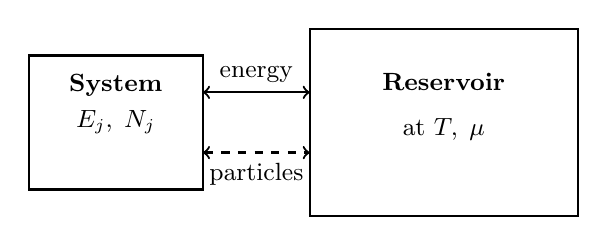
\begin{tikzpicture}[scale=0.85]
  \draw[thick] (0,0) rectangle (2.6, 2.0);
  \node[font=\small\bfseries] at (1.3, 1.55) {System};
  \node[font=\small] at (1.3, 1.0) {$E_j,\; N_j$};
  \draw[thick] (4.2, -0.4) rectangle (8.2, 2.4);
  \node[font=\small\bfseries] at (6.2, 1.6) {Reservoir};
  \node[font=\small] at (6.2, 0.9) {at $T,\;\mu$};
  \draw[<->, thick] (2.6, 1.45) -- (4.2, 1.45)
        node[midway, above, font=\small] {energy};
  \draw[<->, thick, dashed] (2.6, 0.55) -- (4.2, 0.55)
        node[midway, below, font=\small] {particles};
\end{tikzpicture}\\[3pt]
{\small\itshape Grand canonical ensemble: system exchanges both energy and particles with
a reservoir at $T$, $\mu$.}
\end{center}

% ------------------------------------------------------------------
\section{Fermi--Dirac and Bose--Einstein Statistics}
% ------------------------------------------------------------------

\subsection{Factorisation of the Grand Partition Function}

For non-interacting quantum particles, label single-particle levels $\varepsilon_\alpha$.
A many-body microstate is specified by occupation numbers $\{n_\alpha\}$, and
\begin{equation}
    e^{-\beta(E_j - \mu N_j)}
    = \prod_\alpha e^{\beta(\mu-\varepsilon_\alpha)n_\alpha}.
\end{equation}
Summing over all allowed $\{n_\alpha\}$:
\begin{equation}
    \mathcal{Z} = \prod_\alpha \sum_{n_\alpha} e^{\beta(\mu-\varepsilon_\alpha)n_\alpha}
    \equiv \prod_\alpha \mathcal{Z}_\alpha.
\end{equation}
The grand canonical ensemble eliminates the fixed-$N$ constraint, so the occupation sums decouple.

\subsection{Fermions: the Fermi--Dirac Distribution}

For fermions, $n_\alpha \in \{0,1\}$:
\begin{equation}
    \mathcal{Z}_\alpha^{\text{(F)}} = 1 + e^{\beta(\mu-\varepsilon_\alpha)}.
\end{equation}
\begin{formula}
\begin{equation}
    \mathcal{Z} = \prod_\alpha \Bigl(1 + e^{\beta(\mu-\varepsilon_\alpha)}\Bigr).
\end{equation}
\end{formula}
Differentiating $\ln\mathcal{Z}$ with respect to $\mu$ at fixed $\beta$:

\begin{formula}
\textbf{Fermi--Dirac distribution:}
\begin{equation}
    \boxed{\langle n_\alpha \rangle_{\text{FD}}
    = \frac{1}{e^{\beta(\varepsilon_\alpha - \mu)} + 1}.}
\end{equation}
\end{formula}

\subsection{Bosons: the Bose--Einstein Distribution}

For bosons $n_\alpha = 0,1,2,\ldots$; the single-level sum is a geometric series:
\begin{equation}
    \mathcal{Z}_\alpha^{\text{(B)}}
    = \sum_{n_\alpha=0}^\infty e^{\beta(\mu-\varepsilon_\alpha)n_\alpha}
    = \frac{1}{1 - e^{\beta(\mu-\varepsilon_\alpha)}},
\end{equation}
convergent provided $\mu < \varepsilon_\alpha$ for all $\alpha$.
\begin{formula}
\begin{equation}
    \mathcal{Z} = \prod_\alpha \frac{1}{1 - e^{\beta(\mu-\varepsilon_\alpha)}}.
\end{equation}
\end{formula}
Differentiating $\ln\mathcal{Z}$ with respect to $\mu$:

\begin{formula}
\textbf{Bose--Einstein distribution:}
\begin{equation}
    \boxed{\langle n_\alpha \rangle_{\text{BE}}
    = \frac{1}{e^{\beta(\varepsilon_\alpha - \mu)} - 1}.}
\end{equation}
\end{formula}

\subsection{Classical Limit and the Maxwell--Boltzmann Distribution}

When $e^{\beta(\varepsilon_\alpha-\mu)} \gg 1$, both distributions reduce to the classical Maxwell--Boltzmann result $\langle n_\alpha\rangle \approx e^{-\beta(\varepsilon_\alpha - \mu)}$. Quantum corrections matter when $N\lambda_\text{th}^3/V \sim 1$.

\begin{definition}[Quantum Degeneracy Criterion]
A gas is \emph{quantum degenerate} when
\begin{equation}
    \frac{N}{V}\,\lambda_\text{th}^3 \sim 1.
\end{equation}
In the opposite limit $N\lambda_\text{th}^3 \ll V$, the classical
approximation $Z_N = Z_1^N/N!$ applies.
\end{definition}

\begin{center}
\begin{tikzpicture}[scale=0.85]
  \draw[->] (0,0) -- (3.8,0) node[right, font=\small] {$\varepsilon_\alpha$};
  \draw[->] (0,0) -- (0,3.0) node[above, font=\small] {$\langle n_\alpha\rangle$};
  \node[font=\small\bfseries] at (1.9, 3.3) {Quantum degenerate};

  \draw[blue, thick] (0, 2.0) -- (1.8, 2.0)
                     .. controls (1.8,2.0) and (2.0,2.0) .. (2.0, 1.0)
                     .. controls (2.0,1.0) and (2.1,0.0) .. (2.3, 0.0)
                     -- (3.6, 0.0);
  \node[blue, right, font=\scriptsize] at (2.05, 1.6) {FD};

  \draw[red!80!black, thick, domain=0.25:3.6, samples=60]
        plot (\x, {2.0 / (exp(2.5*(\x - 0.4)) - 1) > 2.8 ? 2.8 : 2.0 / (exp(2.5*(\x-0.4))-1)});
  \node[red!80!black, right, font=\scriptsize] at (1.0, 2.55) {BE};

  \draw (1.8, -0.07) -- (1.8, 0.07);
  \node[below, font=\scriptsize] at (1.8, -0.07) {$\varepsilon_F$};
  \node[left, font=\scriptsize] at (0, 2.0) {$1$};

  \begin{scope}[xshift=5.2cm]
    \draw[->] (0,0) -- (3.8,0) node[right, font=\small] {$\varepsilon_\alpha$};
    \draw[->] (0,0) -- (0,3.0) node[above, font=\small] {$\langle n_\alpha\rangle$};
    \node[font=\small\bfseries] at (1.9, 3.3) {Classical limit};
    \draw[green!60!black, thick, domain=0:3.5, samples=60]
          plot (\x, {2.4 * exp(-1.2*\x)});
    \node[green!60!black, right, font=\scriptsize] at (0.5, 1.8) {MB};
    \node[green!60!black, font=\scriptsize] at (2.2, 0.6)
          {$e^{-\beta\varepsilon}$};
  \end{scope}
\end{tikzpicture}\\[3pt]
{\small\itshape Quantum degenerate limit (left): FD step function and BE enhancement.
Classical limit (right): Maxwell--Boltzmann.}
\end{center}

% ------------------------------------------------------------------
\section{The Photon Gas}
% ------------------------------------------------------------------

\subsection{Physical Setup and Allowed Modes}

Photons are bosons with $\mu = 0$ (number not conserved). Allowed standing-wave modes in a cubic box of side $L$:

Standing waves with conducting boundary conditions ($E_\parallel = 0$):
\begin{align}
    E_x &= E_{x0}\cos(k_x x)\sin(k_y y)\sin(k_z z)\sin(\omega t),\notag\\
    E_y &= E_{y0}\sin(k_x x)\cos(k_y y)\sin(k_z z)\sin(\omega t),\\
    E_z &= E_{z0}\sin(k_x x)\sin(k_y y)\cos(k_z z)\sin(\omega t).\notag
\end{align}
Dispersion: $\omega = c|\vec{k}|$.  Transversality $\nabla\cdot\vec{E} = 0$
leaves two independent polarisation states per wavevector.

\begin{formula}
\begin{equation}
    \vec{k} = \frac{\pi}{L}(n_x,\,n_y,\,n_z), \qquad n_x, n_y, n_z = 0, 1, 2, \ldots,
\end{equation}
with two polarisation modes per $\vec{k}$.
\end{formula}

Each mode is a quantum harmonic oscillator with energy levels
$\mathcal{E}_n(\vec{k}) = (n+\tfrac{1}{2})\hbar\omega(\vec{k})$.

\begin{definition}
\begin{equation}
    E(\text{state}) = \sum_{\vec{k},\lambda}
    \left(n_{\vec{k},\lambda}+\tfrac{1}{2}\right)\hbar\omega(\vec{k}).
\end{equation}
\end{definition}

\subsection{Partition Function and Internal Energy}

The partition function factorises over modes:
\begin{equation}
    Z = \prod_{\vec{k},\lambda}\sum_{n=0}^{\infty}
    e^{-\beta(n+\frac{1}{2})\hbar\omega(\vec{k})}
    = \prod_{\vec{k},\lambda} Z_\omega(\vec{k}), \qquad
    Z_\omega = \frac{e^{-\beta\hbar\omega/2}}{1-e^{-\beta\hbar\omega}}.
\end{equation}
In the thermodynamic limit (mode sum $\to$ integral, two polarisations):
\begin{equation}
    \ln Z = \frac{V}{\pi^2 c^3}\int_0^\infty \omega^2
    \left[-\frac{\beta\hbar\omega}{2}
          -\ln\!\left(1-e^{-\beta\hbar\omega}\right)\right]d\omega.
\end{equation}
Dropping the temperature-independent zero-point term:

\begin{formula}
\textbf{Log-partition function of the photon gas:}
\begin{equation}
    \ln Z = -\frac{V}{\pi^2 c^3}\int_0^\infty \omega^2
    \ln\!\left(1-e^{-\beta\hbar\omega}\right)\,d\omega.
\end{equation}
\end{formula}

The internal energy $U = -\partial_\beta \ln Z$:
\begin{equation}
    U = \frac{V}{\pi^2 c^3}\int_0^\infty
    \underbrace{\omega^2}_{\text{density of modes}}\;
    \underbrace{\frac{\hbar\omega}{e^{\beta\hbar\omega}-1}}_{\text{mean energy per mode}}
    \,d\omega.
\end{equation}
Substituting $\tau = \beta\hbar\omega$:
\begin{equation}
    U = \frac{\hbar V}{\pi^2 c^3}\!\left(\frac{k_BT}{\hbar}\right)^{\!4}
    \int_0^\infty \frac{\tau^3\,d\tau}{e^\tau-1}.
\end{equation}

\begin{fact}
\textbf{Riemann zeta function:} $\int_0^\infty x^s (e^x - 1)^{-1}\,dx = s!\;\zeta(s+1)$, so
\begin{equation}
    \int_0^\infty \frac{\tau^3\,d\tau}{e^\tau-1} = 3!\;\zeta(4)
    = 6\cdot\frac{\pi^4}{90} = \frac{\pi^4}{15}.
\end{equation}
Relevant values: $\zeta(2) = \pi^2/6$, $\zeta(3)\approx 1.202$, $\zeta(4) = \pi^4/90$.
\end{fact}

\begin{formula}
\textbf{Stefan's $T^4$ law:}
\begin{equation}
    \frac{U}{V} = \frac{\pi^2 k_B^4}{15\hbar^3 c^3}\,T^4 = \frac{4\sigma}{c}\,T^4,
    \qquad \sigma \equiv \frac{\pi^2 k_B^4}{60\hbar^3 c^2}.
\end{equation}
\end{formula}

From $F = -U/3$ (by integration by parts in the frequency integral):
\begin{equation}
    P = -\pdv{F}{V}\bigg|_T = \frac{U}{3V} = \frac{4\sigma T^4}{3c},
\end{equation}
\begin{formula}
\textbf{Entropy of the photon gas:}
\begin{equation}
    S = -\pdv{F}{T}\bigg|_V = \frac{4U}{3T} = \frac{16\sigma T^3 V}{3c}.
\end{equation}
\end{formula}
Heat capacity $C_V \propto T^3$.  Radiation pressure equals $U/(3V)$, as for
massless particles.  Photon number $N \propto T^3$ adjusts freely with temperature.

\subsection{Stefan--Boltzmann Law and Spectral Radiance}

The spectral power per unit area escaping through a small hole:
\begin{fact}
\begin{equation}
    \frac{P/A}{\text{unit }\omega}
    = \frac{\hbar}{4\pi^2 c^2}\cdot\frac{\omega^3}{e^{\beta\hbar\omega}-1}.
\end{equation}
\end{fact}

\begin{theorem}[Stefan--Boltzmann Law]
\begin{equation}
    \frac{P}{A} = \sigma T^4, \qquad
    \sigma = \frac{\pi^2 k_B^4}{60\hbar^3 c^2} \approx 5.67\times 10^{-8}
    \,\text{W\,m}^{-2}\text{K}^{-4}.
\end{equation}
\end{theorem}


\subsection{Classical Limit and the Ultraviolet Catastrophe}

In the classical limit $e^{\beta\hbar\omega}-1 \approx \beta\hbar\omega$, each mode contributes $k_BT$:
\begin{equation}
    U \to \frac{k_BTV}{\pi^2 c^3}\int_0^\infty \omega^2\,d\omega \to \infty.
\end{equation}
This \textbf{ultraviolet catastrophe} is cured by quantisation: high-frequency modes are exponentially frozen out.

\subsection{Application: Equilibrium Temperature of the Earth}

\begin{example}
Sun: $T_0 \approx 5772\,\text{K}$, $R_\odot \approx 6.96\times 10^8\,\text{m}$;
Earth--Sun distance $a \approx 1.5\times 10^{11}\,\text{m}$.  Power intercepted
by Earth's cross-section equals power radiated by its full surface:
\begin{equation}
    P_\text{in} = 4\pi R_\odot^2\,\sigma T_0^4 \cdot \frac{\pi R_E^2}{4\pi a^2}
    = P_\text{out} = 4\pi R_E^2\,\sigma T_E^4.
\end{equation}

\begin{formula}
\textbf{Earth's radiative equilibrium temperature:}
\begin{equation}
    T_E = T_0\!\left(\frac{R_\odot}{2a}\right)^{\!1/2} \approx 278\,\text{K}.
\end{equation}
The actual surface temperature is higher due to the greenhouse effect.
\end{formula}
\end{example}

% ------------------------------------------------------------------
\section{Degenerate Fermi Systems}
% ------------------------------------------------------------------

\subsection{The Zero-Temperature Fermi Gas}

At $T = 0$, the Fermi--Dirac distribution is a sharp step:
\begin{equation}
    \langle n_\alpha\rangle \xrightarrow{T\to 0}
    \begin{cases}
        1 & \varepsilon_\alpha < \mu, \\
        0 & \varepsilon_\alpha > \mu.
    \end{cases}
\end{equation}
The chemical potential at $T = 0$ is the \textbf{Fermi energy} $\varepsilon_F$;
the surface in energy space at $\varepsilon = \mu$ is the \textbf{Fermi surface}.

\begin{center}
\begin{tikzpicture}[scale=0.85]
  \draw[->] (0,0) -- (5.5,0) node[right, font=\small] {$\varepsilon_\alpha$};
  \draw[->] (0,0) -- (0,3.2) node[above, font=\small] {$\langle n_\alpha\rangle$};

  \draw[gray, dashed] (2.8, 0) -- (2.8, 2.4);
  \node[below, font=\small] at (2.8, 0) {$\varepsilon_F$};

  \draw (-0.07, 2.0) -- (0.07, 2.0);
  \node[left, font=\small] at (0, 2.0) {$1$};
  \draw (-0.07, 1.0) -- (0.07, 1.0);
  \node[left, font=\small] at (0, 1.0) {$\tfrac{1}{2}$};

  \draw[blue!80!black, thick, dashed]
        (0, 2.0) -- (2.8, 2.0) -- (2.8, 0.0) -- (5.2, 0.0);
  \node[blue!80!black, font=\small] at (1.2, 2.3) {$T=0$};

  \draw[red!80!black, thick, domain=0.0:5.2, samples=120]
        plot (\x, {2.0 / (exp(4.0*(\x/2.8 - 1.0)) + 1)});
  \node[red!80!black, font=\small] at (4.2, 1.0) {$T>0$};

  \filldraw[red!80!black] (2.8, 1.0) circle (2.5pt);

  \draw[<->, thick] (2.0, -0.55) -- (3.6, -0.55);
  \node[below, font=\scriptsize] at (2.8, -0.55) {${\sim}k_BT$};
\end{tikzpicture}\\[3pt]
{\small\itshape Fermi--Dirac distribution: step at $T=0$ (dashed), thermally broadened
for $T>0$; $\langle n\rangle=\tfrac{1}{2}$ at $\varepsilon=\varepsilon_F$.}
\end{center}

For spin-$\tfrac{1}{2}$ particles in a box of volume $V$, the density of
states $g(\varepsilon) \propto \sqrt{\varepsilon}$ and normalisation gives
\begin{equation}
    N = \int_0^{\varepsilon_F} g(\varepsilon)\,d\varepsilon \propto \varepsilon_F^{3/2},
\end{equation}
so $\varepsilon_F \propto (N/V)^{2/3}$: denser systems have higher Fermi energies.
At $T = 0$, $\mu(T=0) = \varepsilon_F$.

\subsection{Low-Temperature Corrections: the Sommerfeld Expansion}

For $T \ll T_F \equiv \varepsilon_F/k_B$, a systematic expansion in $k_BT/\varepsilon_F$
gives
\begin{equation}
    U(T) \approx U(0) + \frac{\pi^2}{6}g(\varepsilon_F)(k_BT)^2 + O(T^4),
\end{equation}
and a heat capacity linear in temperature:
\begin{equation}
    C_V \approx \frac{\pi^2}{3}k_B^2 T\, g(\varepsilon_F) \propto T,
\end{equation}
in contrast to the classical $C_V = \tfrac{3}{2}Nk_B$.  This linear-$T$ specific
heat is observed in metals at low temperatures.

\begin{fact}
\textbf{Conduction electrons in metals.}
For copper: $n \approx 8.5\times10^{28}\,\text{m}^{-3}$,
$\varepsilon_F \approx 7\,\text{eV}$, $T_F \approx 81\,000\,\text{K}$.
At room temperature $T/T_F \approx 0.004$: the electron gas is deeply degenerate.
Most electrons cannot be thermally excited because nearby states are occupied.
This physics also underlies the stability of white dwarf stars (electron degeneracy
pressure) and neutron stars (neutron degeneracy pressure).
\end{fact}

% ------------------------------------------------------------------
\section{Bose--Einstein Condensation}
% ------------------------------------------------------------------

\subsection{The Maximum Density of Excited States}

The Bose--Einstein distribution requires $\mu < \varepsilon_0 = 0$.  As $T$
decreases at fixed $N/V$, $\mu$ rises toward $0$.  Setting $\mu = 0$ in the
integral over the three-dimensional density of states $g(\varepsilon) \propto \sqrt{\varepsilon}$:
\begin{equation}
    \frac{N_\text{excited, max}}{V}
    = \frac{2}{\sqrt{\pi}}\cdot\frac{1}{\lambda_\text{th}^3}
      \int_0^\infty \frac{\sqrt{u}\,du}{e^u - 1}
    = \frac{\zeta(3/2)}{\lambda_\text{th}^3},
\end{equation}
where $\zeta(3/2) \approx 2.612$.  The integral converges because $g(\varepsilon)
\propto \sqrt{\varepsilon}$ vanishes faster than the BE divergence at $\varepsilon \to 0$.
At any $T$, excited states hold only a finite density of particles. Since $g(\varepsilon_0) = 0$, the ground state is absent from the continuum integral and must be treated separately.

\subsection{Condensation and the Condensate Fraction}

Total particle number:
\begin{equation}
    N = n_0 + V\lambda_\text{th}^{-3}\,\zeta(3/2).
\end{equation}
When $N/V < \zeta(3/2)/\lambda_\text{th}^3$, all particles fit in excited states
and $n_0 \approx 0$.  As $T$ decreases, $\lambda_\text{th}$ grows until excited
states can no longer hold all $N$ particles; $\mu$ saturates at $0$ and the
remainder condenses into the ground state.

\begin{fact}[Bose--Einstein Condensation]
When $N/V > \zeta(3/2)/\lambda_\text{th}^3$, a macroscopic fraction condenses
into the ground state:
\begin{equation}
    \frac{n_0}{N} = 1 - \left(\frac{T}{T_c}\right)^{3/2},
\end{equation}
where the \textbf{condensation temperature} satisfies
\begin{equation}
    \frac{N}{V} = \frac{\zeta(3/2)}{\lambda_\text{th}^3(T_c)},
    \qquad
    k_BT_c = \frac{2\pi\hbar^2}{m}\!\left(\frac{N}{V\,\zeta(3/2)}\right)^{\!2/3}.
\end{equation}
Below $T_c$, the condensate fraction grows continuously from zero: a phase
transition driven purely by quantum statistics.
\end{fact}

\begin{center}
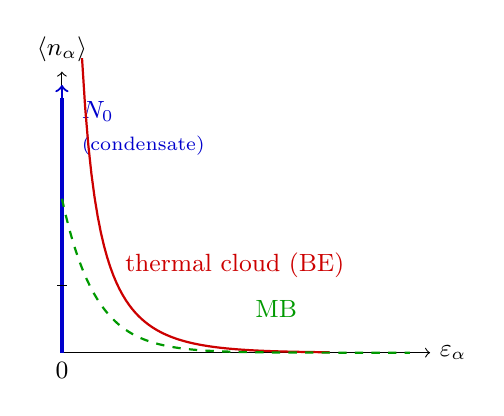
\begin{tikzpicture}[scale=0.85]
  \draw[->] (0,0) -- (5.5,0) node[right, font=\small] {$\varepsilon_\alpha$};
  \draw[->] (0,0) -- (0,4.2) node[above, font=\small] {$\langle n_\alpha\rangle$};
  \node[below, font=\small] at (0, 0) {$0$};

  \draw[blue!80!black, very thick] (0.0, 0.0) -- (0.0, 3.8);
  \draw[blue!80!black, ->, thick] (0.0, 3.8) -- (0.0, 4.0);
  \node[blue!80!black, right, font=\small] at (0.15, 3.6) {$N_0$};
  \node[blue!80!black, font=\scriptsize, right] at (0.15, 3.1) {(condensate)};

  \draw[red!80!black, thick, domain=0.3:4.0, samples=80]
        plot (\x, {2.5 / (exp(1.5*\x) - 1)});
  \node[red!80!black, right, font=\small] at (0.8, 1.3) {thermal cloud (BE)};

  \draw[green!60!black, thick, dashed, domain=0.0:5.2, samples=100]
        plot (\x, {2.3 * exp(-2.0*\x)});
  \node[green!60!black, font=\small] at (3.2, 0.65) {MB};

  \draw (-0.07, 1.0) -- (0.07, 1.0);
\end{tikzpicture}\\[3pt]
{\small\itshape BEC: macroscopic ground-state occupation $N_0$ (spike) plus a thermal BE tail.}
\end{center}

BEC is a purely quantum-statistical effect in an ideal gas, driven by bosonic clustering. First observed in 1995 (Cornell, Wieman, Ketterle) in dilute alkali gases at $\sim 100\,\text{nK}$; condensates show long-range phase coherence and quantised vortices.
